%! BibTeX Compiler = biber
%TC:ignore
\documentclass{article}

\usepackage{xcolor, colortbl}
\definecolor{BLUELINK}{HTML}{0645AD}
\definecolor{DARKBLUELINK}{HTML}{0B0080}
\definecolor{LIGHTGREY}{gray}{0.9}
\PassOptionsToPackage{hyphens}{url}
\usepackage[colorlinks=false]{hyperref}
% for linking between references, figures, TOC, etc in the pdf document
\hypersetup{colorlinks,
    linkcolor=DARKBLUELINK,
    anchorcolor=DARKBLUELINK,
    citecolor=DARKBLUELINK,
    filecolor=DARKBLUELINK,
    menucolor=DARKBLUELINK,
    urlcolor=BLUELINK
} % Color citation links in purple
\PassOptionsToPackage{unicode}{hyperref}
\PassOptionsToPackage{naturalnames}{hyperref}

\usepackage{biorxiv}
\usepackage[backend=biber,eprint=false,isbn=false,url=false,intitle=true,style=nature,date=year]{biblatex}
\addbibresource{codon_models.bib}

\usepackage{url}
\usepackage{amssymb,amsfonts,amsmath,amsthm,mathtools}
\usepackage{lmodern}
\usepackage{xfrac, nicefrac}
\usepackage{bm}
\usepackage{listings, enumerate, enumitem}
\usepackage[export]{adjustbox}
\usepackage{graphicx}
\usepackage{bbold}
\usepackage{pdfpages}
\pdfinclusioncopyfonts=1
\usepackage{lineno}
\usepackage{tabu}
\usepackage{hhline}
\usepackage{multicol,multirow,array}
\usepackage{etoolbox}
\usepackage{booktabs}
\usepackage{makecell}
\usepackage{orcidlink}

\newcommand{\NS}[1]{\textcolor{red}{\textbf{\emph{[NS: #1]}}}}

\newcommand{\UniDimArray}[1]{\bm{#1}}
\newcommand{\der}{\text{d}}
\newcommand{\e}{\text{e}}
\newcommand{\Ne}{N_{\text{e}}}
\newcommand{\proba}{\mathbb{P}}
\newcommand{\pfix}{\proba_{\text{fix}}}
\newcommand{\dn}{d_N}
\newcommand{\ds}{d_S}
\newcommand{\dnds}{\dn / \ds}
\newcommand{\Sphy}{S_{0}}
\newcommand{\SphyDel}{\mathcal{D}_0}
\newcommand{\SphyNeu}{\mathcal{N}_0}
\newcommand{\SphyBen}{\mathcal{B}_0}
\newcommand{\Sphyclass}{x}
\newcommand{\SphyclassAlt}{y}
\newcommand{\given}{\mid}
\newcommand{\Spop}{S}
\newcommand{\SpopDel}{\mathcal{D}}
\newcommand{\SpopNeu}{\mathcal{N}}
\newcommand{\SpopBen}{\mathcal{B}}
\newcommand{\ProbaPopDel}{\proba [ \SpopDel]}
\newcommand{\ProbaPopNeu}{\proba [ \SpopNeu ]}
\newcommand{\ProbaPopBen}{\proba [ \SpopBen ]}
\newcommand{\AdvMean}{\beta_b}
\newcommand{\DelMean}{\beta_d}
\newcommand{\thetaSyn}{\theta_{\text{S}}}
\renewcommand{\baselinestretch}{1.5}
\renewcommand{\arraystretch}{0.6}
\linenumbers
\frenchspacing

\title{Mammalian protein-coding genes exhibit widespread beneficial mutations that are not adaptive}
\rhead{\scshape Beneficial yet non-adaptive mutations}

\author{
    \large
    \textbf{T. {Latrille}$^{1\dag}$\orcidlink{0000-0002-9643-4668}, J. {Joseph}$^{2\dag}$, D.~A. {Hartasánchez}$^{1}$\orcidlink{0000-0003-2596-6883}, N. {Salamin}$^{1}$\orcidlink{0000-0002-3963-4954}}\\
    \normalsize
    $^{1}$Department of Computational Biology, Université de Lausanne, Lausanne, Switzerland\\
    $^{2}$Laboratoire de Biométrie et Biologie Evolutive, UMR5558, Université Lyon 1, Villeurbanne, France \\
    $^{\dag}$These authors contributed equally to this work\\
    \texttt{\href{mailto:thibault.latrille@ens-lyon.org}{thibault.latrille@ens-lyon.org}} \\
}

% The submission checklist is available at:
% https://docs.google.com/document/d/1aHCF1on0mHTK2DoroPCLP_xto4xwHnGJCGwaL1Vm2UE/edit?usp=sharing

\begin{document}
    \maketitle

%TC:endignore
    \begin{abstract}
        Mutations can be beneficial by bringing innovation to their bearer, allowing them to adapt to environmental change.
        However, mutations can also be beneficial because they are reverting previous deleterious changes, simply restoring pre-existing functions.
        By integrating phylogenomic and population data in mammals, we estimated the contribution of beneficial back-mutations to molecular evolution, which had remained widely overlooked so far.
        Applying a mutation-selection model, we estimated amino acid fitness landscapes for mammalian protein-coding genes.
        Assuming these fitness landscapes do not change, any beneficial mutation is necessarily a back-mutation.
        We confirmed that these beneficial back-mutations are positively selected in extant populations and demonstrated that a substantial part of ongoing positive selection is not driven by adaptation to environmental change.
    \end{abstract}

    \keywords{Adaptation \and Back-mutations \and Phylogenetics \and Population-genetics \and Codon models }

    Adaptation is one of the main processes shaping the diversity of forms and functions across the tree of life~\cite{darwin_origin_1859}.
    Evolutionary adaptation is tightly linked to environmental change and species responding to this change~\cite{merrell_adaptive_1994, gavrilets_adaptive_2009}.
    For adaptation to occur, there must be variation within populations, which mostly appears via mutations in the DNA sequence.
    While neutral mutations will not impact an individual's fitness, deleterious mutations have a negative effect, and beneficial mutations improve their bearer's fitness.
    A beneficial mutation is thus more likely than a neutral mutation to invade the population and reach fixation, resulting in a substitution at the species level.
    Upon environmental change, because adaptive beneficial mutations toward new fitness optima are more likely, the number of substitutions also increases (fig.~\ref{fig:fitness-landscape}A).
    An increased substitution rate is thus commonly interpreted as a sign of adaptation~\cite{mcdonald_adaptative_1991, smith_adaptive_2002, welch_estimating_2006}.
    The availability of large-scale genomic data and the development of theoretical models have enabled the detection and quantification of substitution rate changes across genes and lineages~\cite{yang_statistical_2000, eyre-walker_genomic_2006, moutinho_variation_2019}.
    These approaches, now common practice in evolutionary biology, helped better understand the processes underpinning the rates of molecular evolution.
    However, a collateral effect has been conflating beneficial mutations with adaptive evolution when adaptive evolution is not the only process that can lead to beneficial mutations~\cite{charlesworth_other_2007, mustonen_fitness_2009}.

    In a constant environment, a deleterious mutation can reach fixation by genetic drift~\cite{Ohta1992}.
    A new mutation restoring the ancestral fitness will thus be beneficial (fig.~\ref{fig:fitness-landscape}B), even though the environment has not changed~\cite{hartl_compensatory_1996, sella_application_2005, mustonen_fitness_2009, cvijovic_fate_2015}.
    The restoration of the ancestral fitness can either happen through a mutation at a different locus –~called a compensatory mutation~\cite{hartl_compensatory_1996, mustonen_fitness_2009}, or at the locus of the initial mutation –~called a beneficial back-mutation~\cite{piganeau_estimating_2003, charlesworth_other_2007}.
    While compensatory mutations change the sequence and thus induce genetic diversification, beneficial back-mutations reduce genetic diversity and do not contribute to genetic innovation.
    Although Tomoko Ohta considered beneficial back-mutations negligible in her nearly-neutral theory~\cite{Ohta1992}, their importance has now been acknowledged for expanding populations~\cite{charlesworth_other_2007}.
    However, differentiating between an adaptive mutation and a beneficial back-mutation remains challenging~\cite{chi_detecting_2020}.
    Indeed, an adaptive mutation responding to a change in the environment and a beneficial back-mutation have equivalent consequences for their bearer~\cite{charlesworth_other_2007}.
    Similarly, at the population level, both types of mutations will result in a positive transmission bias of the beneficial allele.
    However, at the macro-evolutionary scale, the consequences of these two types of mutations are fundamentally different.
    While adaptive mutations promote phenotype diversification (fig.~\ref{fig:fitness-landscape}C), beneficial back-mutations promote phenotype stability and may help preserve well-established biological systems (fig.~\ref{fig:fitness-landscape}D).
    Additionally, the direction of adaptive evolution is unpredictable because it is caused by an unforeseen change in the environment and, hence, in the underlying fitness landscape~\cite{bazykin_changing_2015}.
    On the other hand, beneficial back-mutations are predictable if the underlying stable fitness landscape is known because changes from non-optimal amino acids to optimal ones will be expected.

    %In this study, we seek empirical evidence for beneficial back-mutations and test long-standing related questions, such as how common they are and what the probability is for any beneficial mutation observed in current populations to be a back-mutation.
    %By addressing these questions, we provide novel insight into the process of adaptation and, more broadly, into how natural selection has affected protein-coding DNA sequences throughout evolution.
    \subsection*{Fitness landscape reconstruction}
    The mutation-selection framework permits to link the patterns of substitution along a phylogeny with the underlying fitness landscape~\cite{halpern_evolutionary_1998, mccandlish_modeling_2014}.
    Such mutation-selection models applied to protein-coding DNA sequences allow us to estimate relative fitnesses for all amino acids for each site of the sequence, explicitly assuming that the underlying fitness landscape is stable along the phylogenetic tree~\cite{rodrigue_mechanistic_2010, tamuri_estimating_2012, rodrigue_detecting_2017}.
    Importantly, because mutation-selection models at the phylogenetic scale are based on population-genetics equations, their estimates of selection coefficients are directly interpretable as fitness effects for an individual within a population.
    %These methods account for phylogenetic relationships, the structure of the genetic code and accommodate for underlying mutational biases~\cite{rodrigue_mechanistic_2010, tamuri_estimating_2012, latrille_improved_2022}.

    Theoretically, we can thus use large-scale genomic data to assess whether the fitnesses estimated at the phylogenetic scale predict the fitness effect at the population scale for both deleterious and beneficial back-mutations.
    The placental mammals represent an excellent study system to perform such analysis.
    Having originated $\sim$100 million years ago~\cite{kumar_timetree_2017}, they diversified quickly.
    Additionally, polymorphism data are available for many species~\cite{howe_ensembl_2021}, as are high quality protein-coding DNA alignments across the genome~\cite{ranwez_orthomam_2007, scornavacca_orthomam_2019}.
    By restricting our analysis to protein-coding orthologous genes, we focus on genes under functional constrains across mammals.
    For each gene, fitting the mutation-selection model to the multi-species sequence alignment, assuming that the underlying fitness landscape is stable along the phylogenetic tree, allows us to obtain relative fitnesses for all amino acids for each site of the alignment (fig.~\ref{fig:method}A).
    From the fitness landscape, we can calculate the scaled selection coefficient ($\Sphy$) for any possible amino acid change at each position.
    According to its $\Sphy$ value, we can classify any mutation as either a deleterious mutation toward a less fit amino acid ($\SphyDel \coloneqq \Sphy < -1$), a nearly-neutral mutation ($\SphyNeu \coloneqq -1 < \Sphy <1$) or a beneficial back-mutation toward a known fitter amino acid ($\SphyBen \coloneqq \Sphy > 1$).
    Having identified which potential DNA changes represent beneficial back-mutations (fig.~\ref{fig:method}B), we retrieved polymorphism data from 28 populations belonging to 6 genera (\textit{Equus}, \textit{Bos}, \textit{Capra}, \textit{Ovis}, \textit{Chlorocebus}, and \textit{Homo}) to assess the presence of beneficial back-mutations at the population scale.
    We focused on mutations currently segregating within populations and substitutions in the terminal branches, and checked if any of these observed changes were beneficial back-mutations (fig.~\ref{fig:method}C-E).
    In this study, by integrating large-scale genomic datasets at both phylogenetic and population scales, we have been able to estimate the number of beneficial back-mutations across the entire exome of the six genera (figs.~\ref{fig:method}F-G).

    \begin{figure*}[!ht]
        \centering
        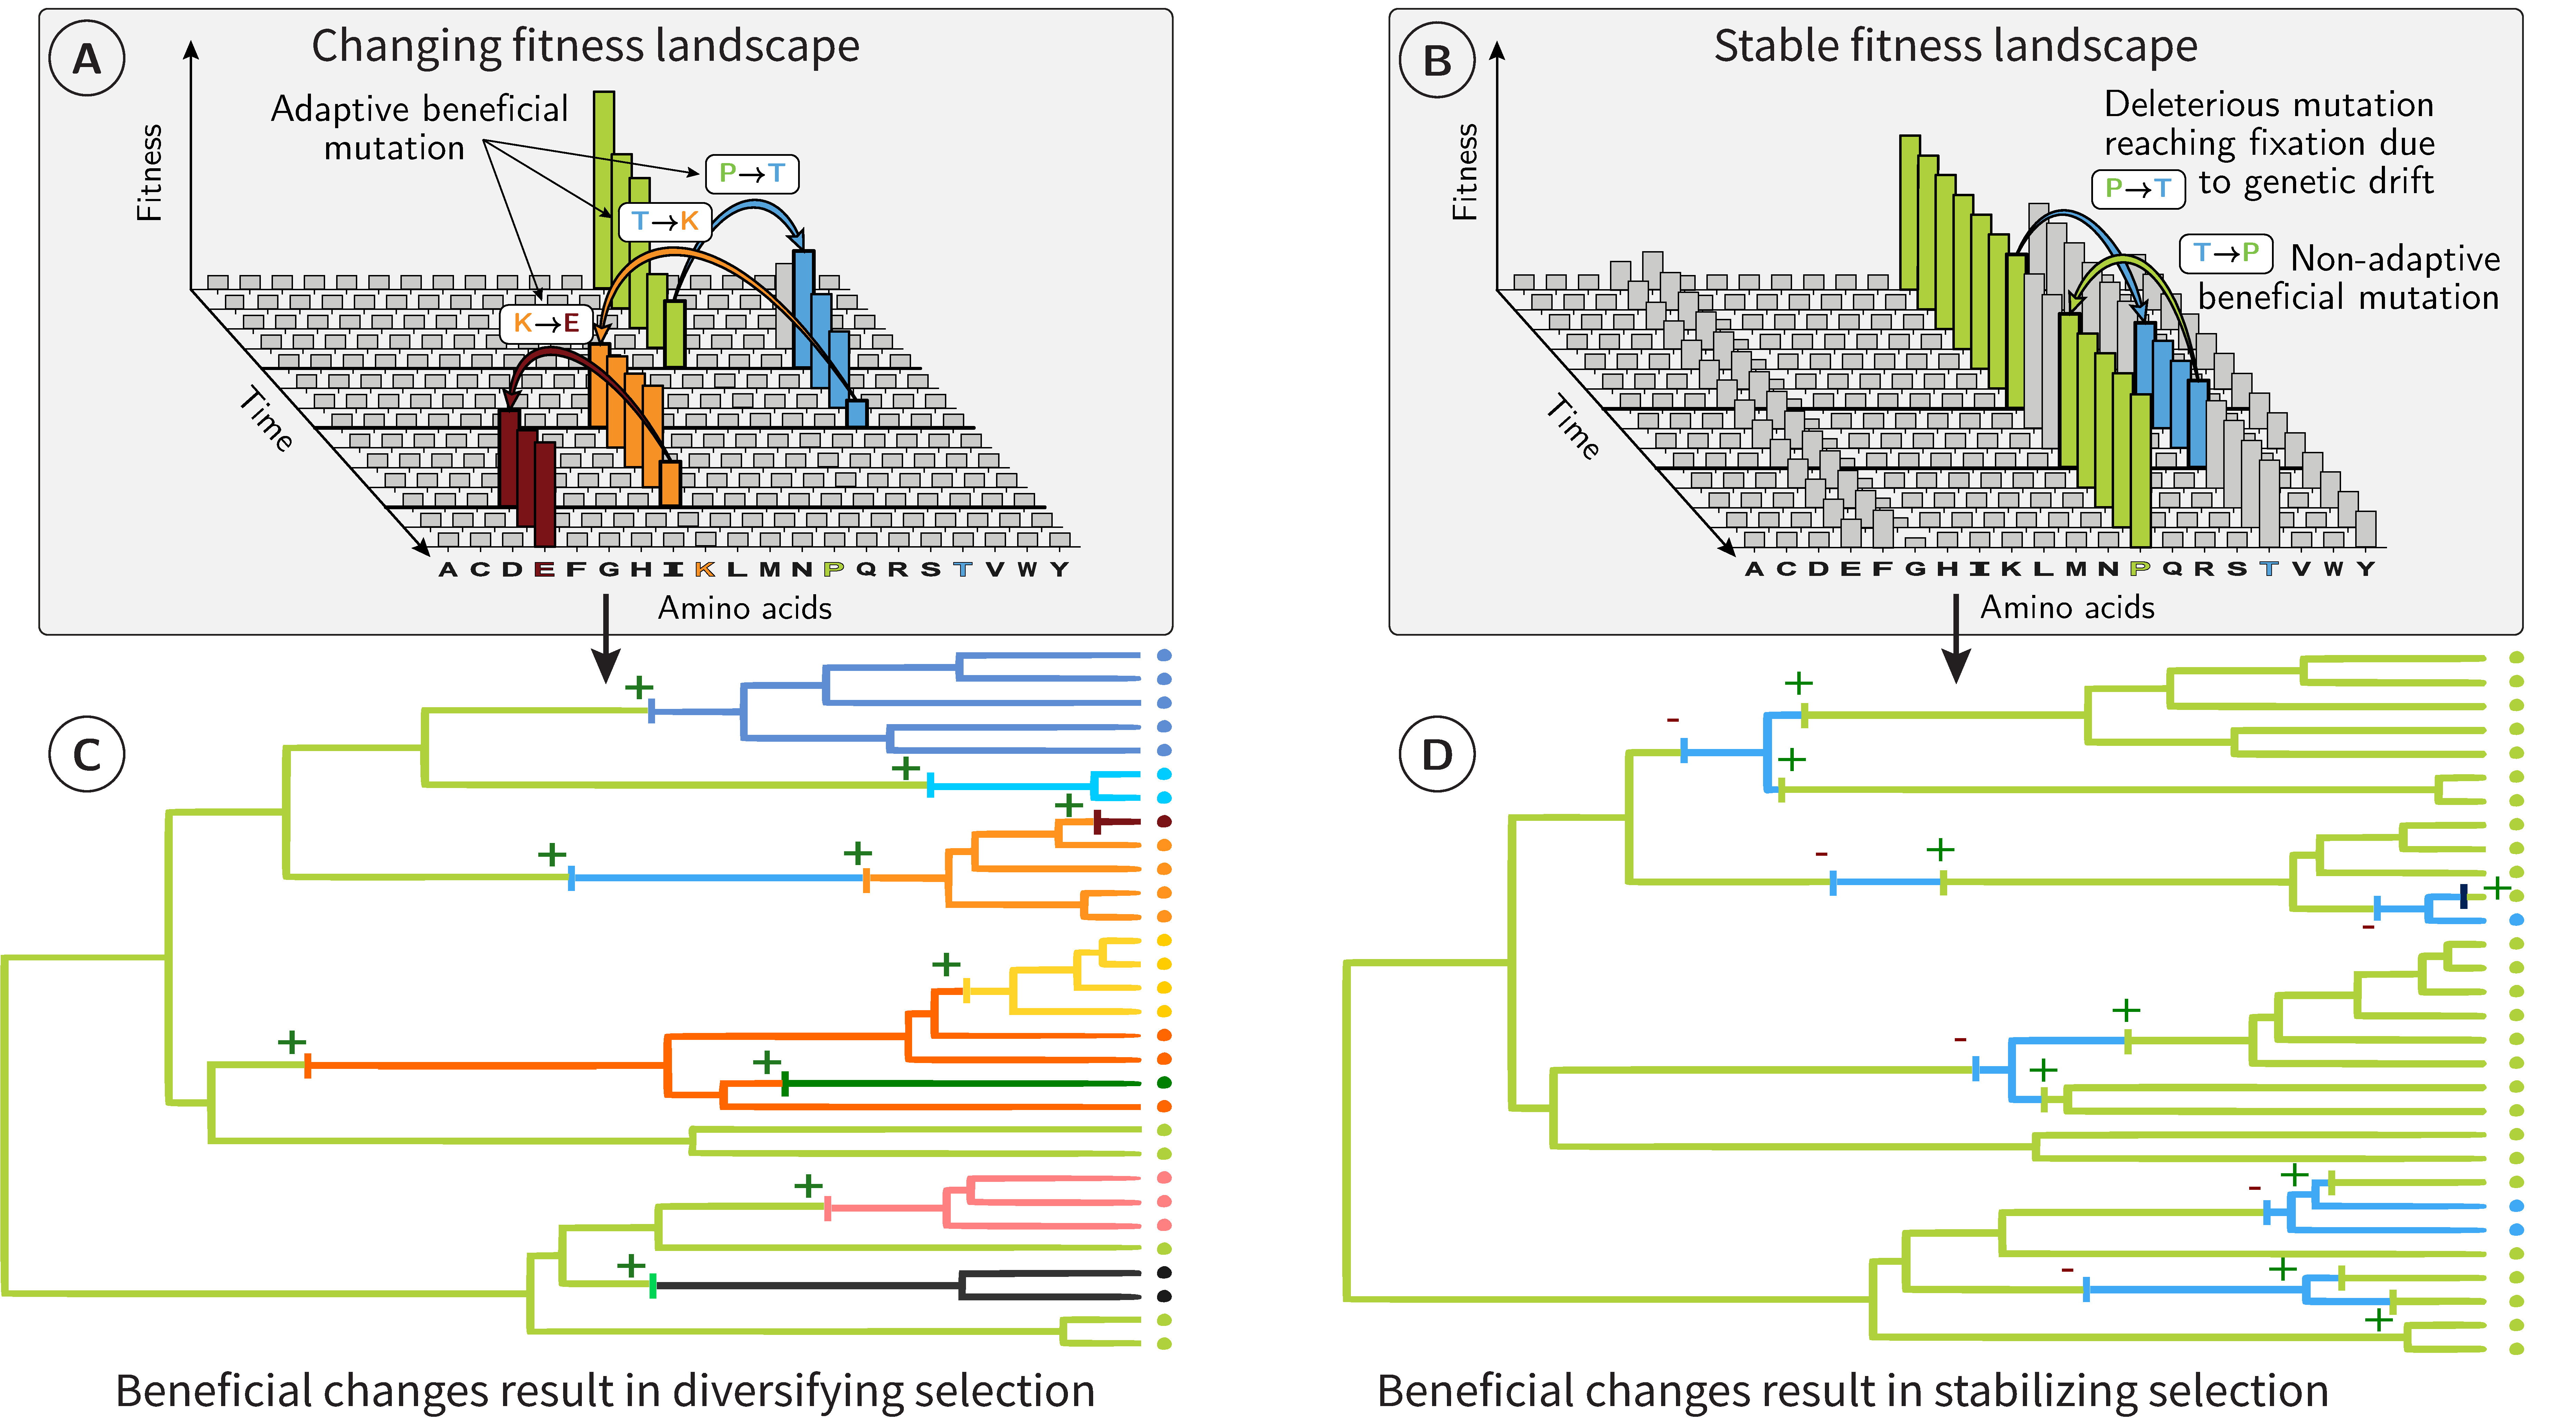
\includegraphics[width=\textwidth, page=1] {artworks/figure.fitness-landscape}
        \caption{
            (A \& B) For a given codon position of a protein-coding DNA sequence, amino acids (x-axis) have different fitness values (y-axis).
            Under a fluctuating fitness landscape (A), these fitnesses change with time.
            The protein sequence follows the moving target defined by the amino-acid fitnesses. Since substitutions are preferentially accepted if they are in the direction of this target, substitutions are, on average, adaptive.
            At the phylogenetic scale (C), beneficial substitutions are common (positive signs), promoting phenotype diversification across species.
            Under a stable fitness landscape (B), most mutations reaching fixation are either slightly deleterious reaching fixation due to drift or are beneficial back-mutations restoring a more optimal amino acid.
            At the phylogenetic scale (D), deleterious substitutions (negative signs) are often reverted via beneficial back-mutations (positive signs), promoting phenotype stability and preserving well-established biological systems.
            Even though, individually, any back-mutation might have a small beneficial effect on its bearer, we expect beneficial back-mutations to be scattered across the genome and the genome-wide signature of beneficial back-mutations to be detectable and quantifiable.}
        \label{fig:fitness-landscape}
    \end{figure*}

    \begin{figure*}[!ht]
        \centering
        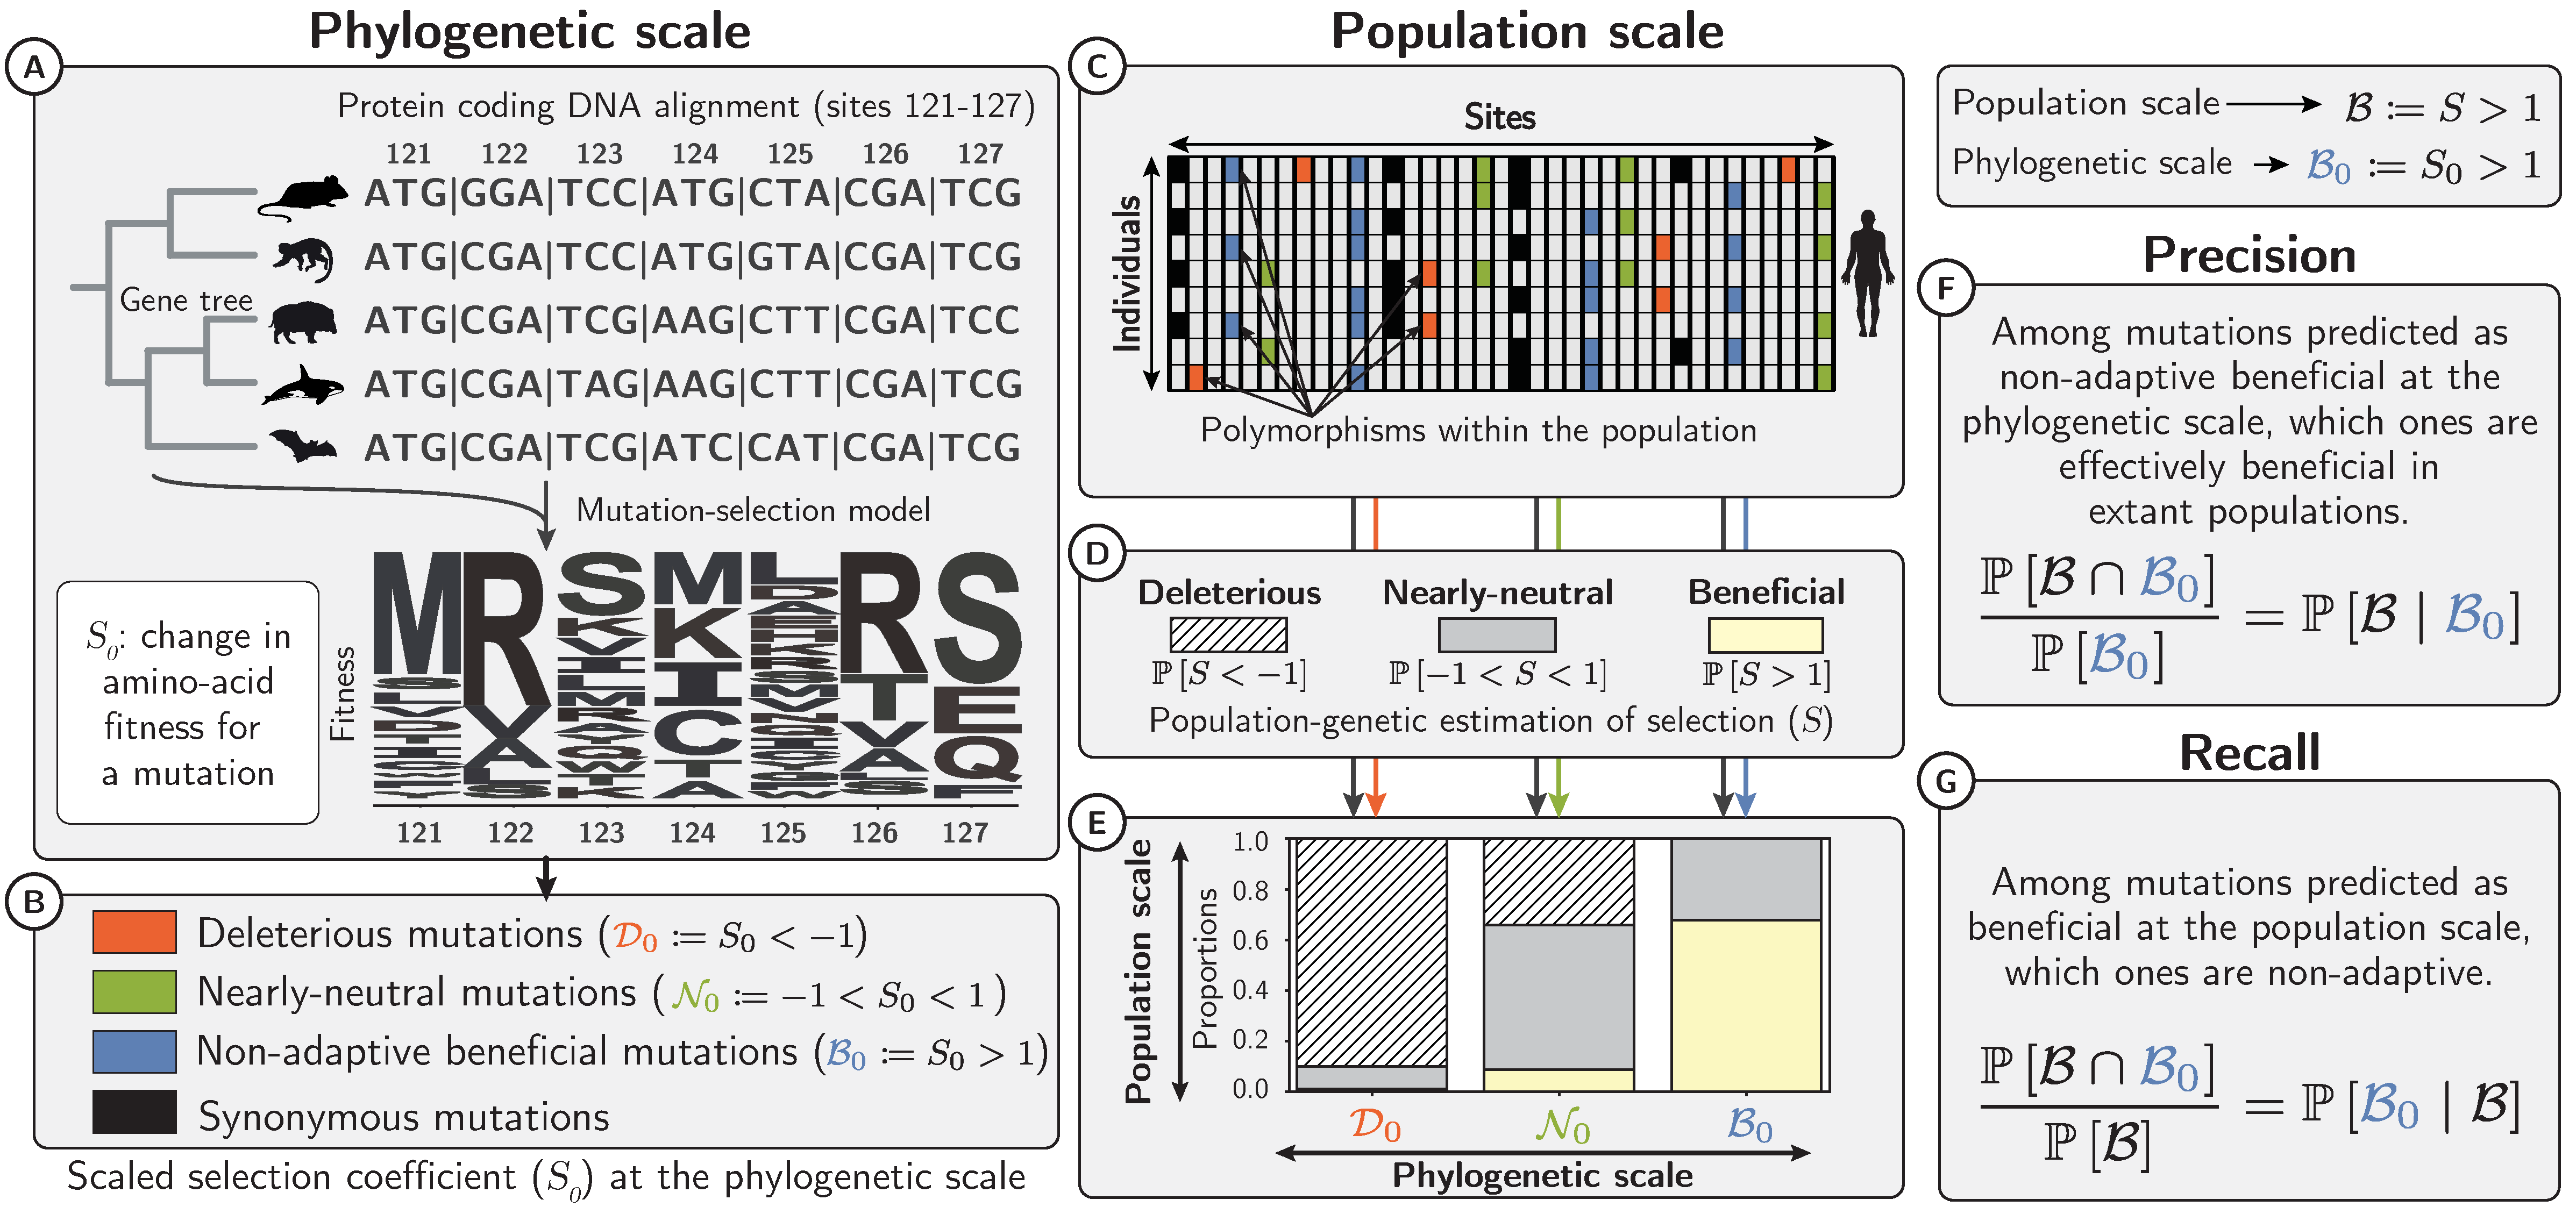
\includegraphics[width=\textwidth, page=1] {artworks/figure.method.proba}
        \caption{
            Selection coefficients at the phylogenetic and population scales.
            At the phylogenetic scale (A), we estimated the amino-acid Wrightian fitness for each site from protein-coding DNA alignments using mutation-selection codon models.
            For every possible mutation, the difference in amino acid fitness before and after the mutation allows us to compute the selection coefficient at the phylogenetic scale ($\Sphy$).
            Depending on $\Sphy$ (B) mutations can be predicted as deleterious ($\SphyDel$), nearly-neutral ($\SphyNeu$) or beneficial back-mutations ($\SphyBen$) toward a fitter amino acid and repairing existing functions.
            Substitutions along the terminal branch are classified depending on their $\Sphy$ value (C).
            At the population scale, each observed single nucleotide polymorphism (SNP) segregating in the population can also be classified according to its $\Sphy$ value.
            Occurence and frequency in the population of non-synonymous and synonymous (deemed neutral) polymorphisms (D-E) is used to estimate selection coefficients at the population scale ($\Spop$), for each class of selection ($\SphyDel$, $\SphyNeu$, $\SphyBen$).
            We can thus assess whether $\Sphy$ predicts $\Spop$ and compute \textit{precision} (F) and \textit{recall} (G) for each class.
            The \textit{recall} value for class $\SphyBen$ is the probability of back-mutations among all beneficial ones (G).
        }
        \label{fig:method}
    \end{figure*}

    \subsection*{Selection along the terminal branches}
    First, we assessed whether fitness effects derived from the mutation-selection model at the phylogenetic scale predict selection occurring in terminal branches.
    We recovered the mutations that reached fixation in the terminal branches of the six genera.
    We only considered mutations fixed in a population as substitutions in the corresponding branch and discarded segregating mutations.
    We classified each substitution identified in the terminal branches as either $\SphyDel$, $\SphyNeu$, or $\SphyBen$ depending on its $\Sphy$ value obtained at the phylogenetic scale (fig.~\ref{fig:method}A-C).
    Importantly, the mammalian alignment used to estimate the amino acid fitness landscape did not include the genera for which we reconstructed the substitutions to avoid fallacy and circular reasoning.
    Because $\Sphy$ was based on estimating fitness effects at the mammalian scale, mutations with $\Sphy>1$ were considered beneficial back-mutations ($\SphyBen$) toward a fitter amino acid.
    Among all the substitutions found in each terminal branch, between 10 and 13\% were $\SphyBen$ (table~S1 and fig.~\ref{fig:homo-afr-results}B for humans).
    In principle, beneficial back-mutations are bound to reach fixation more often than neutral mutations.
    Hence, we calculated the $\dnds$ ratio of non-synonymous over synonymous divergence for all terminal lineages, focusing on the non-synonymous changes predicted as beneficial back-mutations ($\dn(\SphyBen) / \ds$).
    We obtained values between 1.10 and 1.61 in the different lineages (table~S1), implying that $\SphyBen$ mutations reached fixation more frequently than synonymous mutations that are supposed to be neutral, implying that these back-mutations are effectively beneficial.

    This result further indicated that using $\dnds$ as an estimate of adaptation is biased due to the presence of beneficial back-mutations among the non-synonymous substitutions.
    By discarding all beneficial back-mutations we can obtain an estimate of $\dnds$ which is not inflated.
    By comparing these two ways of calculating $\dnds$ (see section~\ref{subsec:substitution-mapping-in-the-terminal-branch} in Materials \& Methods), we calculated that beneficial back-mutations inflate $\dnds$ values by between 9 and 11\% across genera while only representing between 1.2 and 1.4\% of non-synonymous mutations (table~S2-3 and fig.~\ref{fig:homo-afr-results}A for humans).

    \subsection*{Selection in populations}
    Second, we assessed whether our calculated $\Sphy$ values are also indicative of the selective forces exerted at the population level.
    So, we retrieved single nucleotide polymorphisms (SNPs) segregating in 28 mammalian populations.
    To determine if SNPs were ancestral of derived, we reconstructed the ancestral genome of each population.
    We then classified every non-synonymous SNP as either $\SphyDel$, $\SphyNeu$, or $\SphyBen$ according its $\Sphy$ value (fig.~\ref{fig:method}B-C).

    In humans, some SNPs have been associated with specific clinical prognosis terms~\cite{landrum_clinvar_2018} obtained by clinical evaluation of the impact of variants on human Mendelian disorders~\cite{landrum_clinvar_2018}.
    Thus, they provide an orthogonal estimate of the effect of a mutation on human health, allowing us to evaluate whether this effect follows its predicted fitness effect.
    Therefore, we investigated whether the non-synonymous SNPs classified as $\SphyDel$ or $\SphyBen$ showed enrichment in specific clinical terms compared to SNPs classified as $\SphyNeu$.
    Our results show that SNPs predicted as deleterious are associated with clinical terms such as \textit{Likely Pathogenic} and \textit{Pathogenic}, implying that, in general, the selective pressure of a mutation exerted across mammals is also predictive of its clinical effect in humans (table~S4).
    Conversely, back-mutations are associated with clinical terms such as \textit{Benign} and \textit{Likely Benign}, which shows that back-mutations are less likely to be functionally damaging (table~S5).

    In addition to clinical prognosis, frequencies at which SNPs are segregating within populations provide information on their selective effects.
    For instance, deleterious SNPs usually segregate at lower frequencies because of purifying selection, which tends to remove them from the population (fig.~\ref{fig:homo-afr-results}C for humans).
    By gathering information across many SNPs, it is possible to estimate the distribution of fitness effects (DFE) at the population scale, taking synonymous SNPs as a neutral expectation~\cite{eyre-walker_distribution_2006, eyre-walker_estimating_2009, galtier_adaptive_2016, tataru_inference_2017}.
    From the estimated DFE, we can derive the proportion of beneficial mutations ($\ProbaPopBen$), nearly-neutral mutations ($\ProbaPopNeu$) and deleterious mutations ($\ProbaPopDel$) at the population scale (see section~\ref{subsec:s-polymorphism-method} in Materials \& Methods).
    These approaches offer a unique opportunity to contrast selection coefficients estimated at the population scale ($\Spop$) and at the phylogenetic scale ($\Sphy$).

    Across our selection classes ($\SphyDel$, $\SphyNeu$ and $\SphyBen$), one can ultimately estimate the proportion of correct and incorrect predictions, leading to an estimation of \textit{precision} and \textit{recall} (fig.~\ref{fig:method}F-G and section~\ref{subsec:precisison_recall} in Materials \& Methods).
    Across 28 populations of different mammal species, mutations predicted to be deleterious at the phylogenetic scale ($\ProbaPopDel$) were indeed purged at the population scale, with a \textit{precision} in the range of 89--96\% (table~\ref{table:proba} and fig.~\ref{fig:homo-afr-results}D for humans).
    Conversely, a \textit{recall} in the range of 95--100\% implies that mutations found to be deleterious at the population scale were most likely also predicted to be deleterious at the phylogenetic scale (table~\ref{table:proba}).
    Altogether, purifying selection is largely predictable and amino acids with negative fitness across mammals have been effectively purged away in each population.

    Mutations predicted as $\SphyNeu$ were effectively composed of a mix of neutral and selected mutations with varying \textit{precision} (36--73\%) and \textit{recall} (30--45\%) across the different populations (table~\ref{table:proba}, fig.~\ref{fig:homo-afr-results}D for Humans).
    The variable proportions between populations can be explained by the effective number of individuals in the population ($\Ne$), a major driver of selection efficacy.
    Since $\Ne$ is not directly measurable, we used Watterson's $\thetaSyn$ as a proxy to order populations by their levels of synonymous diversity.
    Higher synonymous diversity was associated with a smaller proportion of nearly-neutral mutations (fig.~\ref{fig:diversity}A).
    This result follows the prediction of the nearly-neutral theory and suggests that in populations with higher diversity (e.g.,~\textit{Bos} or \textit{Ovis}), discrimination between beneficial and deleterious mutations is more likely to occur (figs.~S1-S9).
    Conversely, many more mutations are effectively neutral in populations with lower diversity (e.g.,~\textit{Homo}).

    Finally, mutations predicted to be beneficial back-mutations based on the selection coefficients at the phylogenetic scale ($\SphyBen$) were indeed beneficial for individuals bearing them, with a \textit{precision} (fig.~\ref{fig:method}F) in the range of 15--86\% (table~\ref{table:proba} and fig.~\ref{fig:homo-afr-results}D for humans).
    This result confirms that selection towards amino acids restoring existing functions is ongoing in these populations.
    Importantly, the \textit{recall} value in this case, computed as $\proba [ \SphyBen  \given  \SpopBen]$, is the probability for a beneficial mutation at the population scale to be a beneficial back-mutation, i.e., going toward a fitter amino acid (fig.~\ref{fig:method}G).
    In other words, the \textit{recall} value quantifies the number of beneficial mutations restoring damaged genomes instead of creating adaptive innovations.
    Across the 28 populations, this proportion is in the range of 13--80\% (table~\ref{table:proba}).


    \begin{figure*}[!ht]
        \centering
        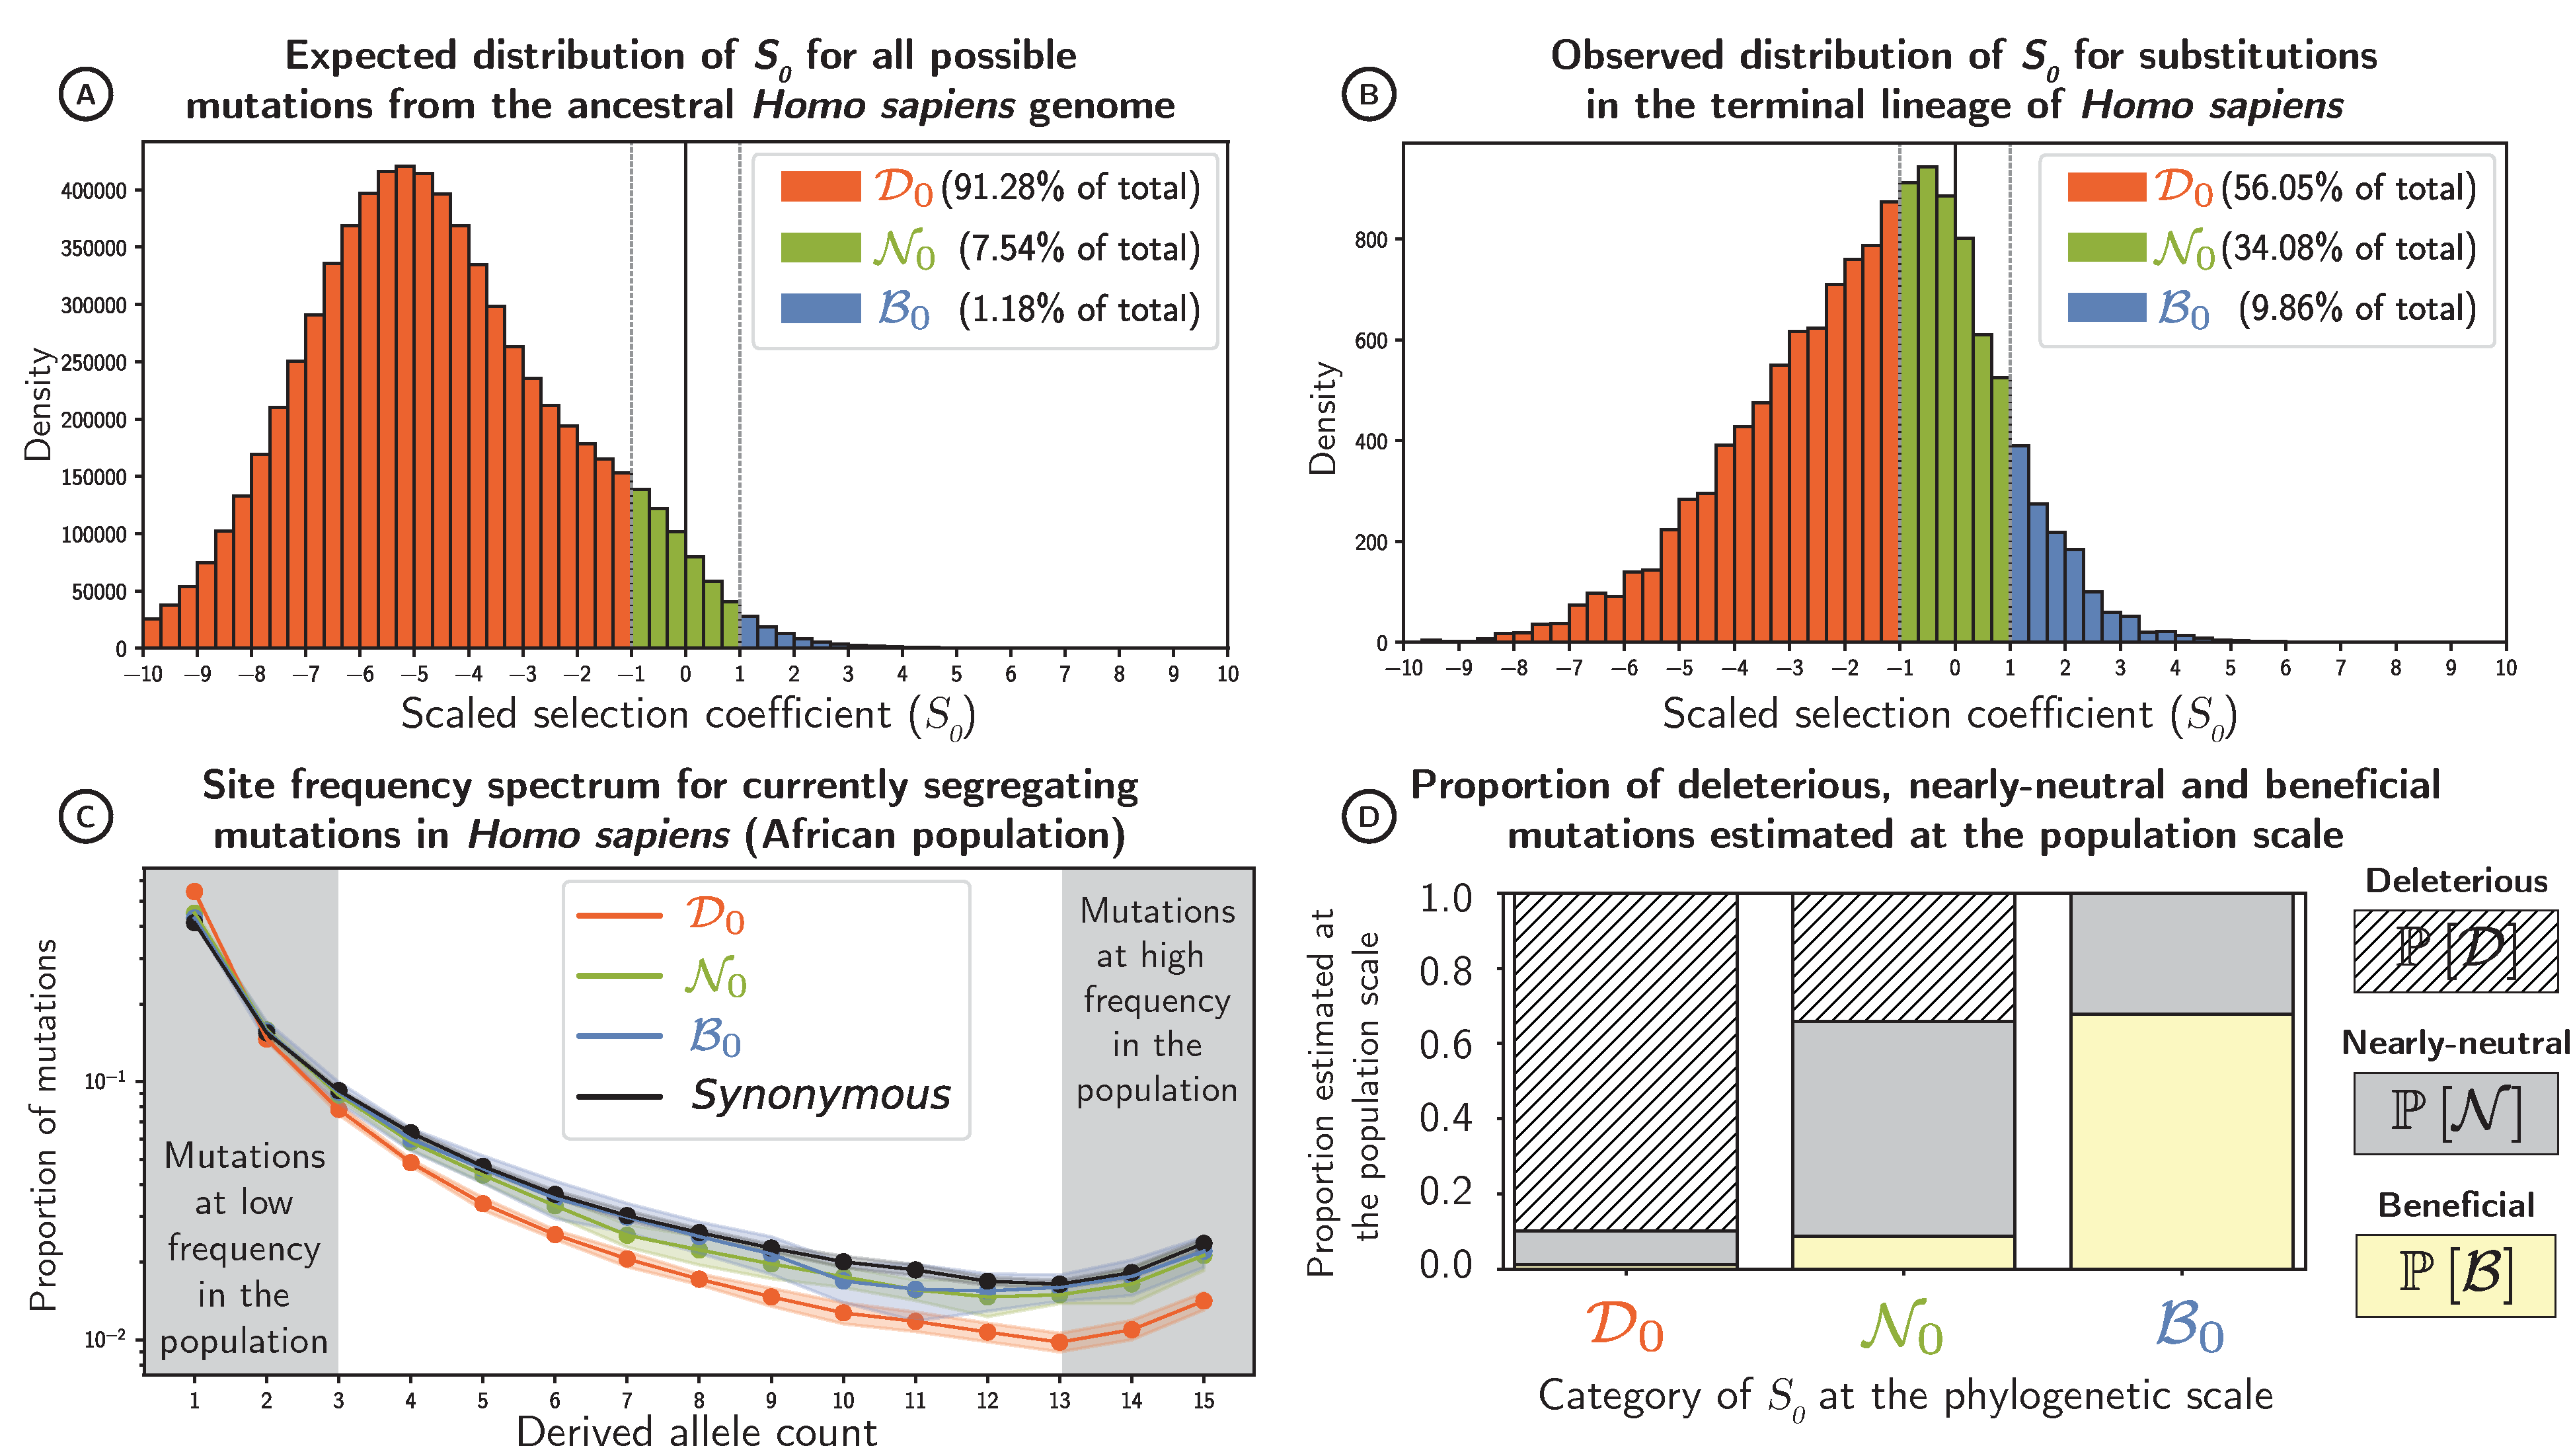
\includegraphics[width=\textwidth, page=1] {artworks/figure.homo-afr-results}
        \caption{
            (A) Distribution of scaled selection coefficients ($\Sphy$), predicted for all possible mutations away from the ancestral human genome.
            Mutations are divided into three classes of selection: deleterious ($\SphyDel$), nearly-neutral ($\SphyNeu$) and beneficial ($\SphyBen$, supposedly beneficial back-mutations).
            (B) Distribution of scaled selection coefficients ($\Sphy$) for all observed substitutions along the \textit{Homo} branch after the \textit{Homo}-\textit{Pan} split.
            If there are fewer substitutions than expected, this class is thus undergoing purifying selection, as is the case for $\SphyDel$.
            (C) The site-frequency spectrum (SFS) in humans of African descent for a random sample of 16 alleles (means in solid lines and standard deviations in color shades) for each class of selection and for synonymous mutations, supposedly neutral (black). The SFS represents the proportion of mutations (y-axis) with a given number of derived alleles in the population (x-axis).
            At high frequencies, deleterious mutations are underrepresented.
            (D) Proportion of beneficial $\ProbaPopDel$, nearly-neutral $\ProbaPopNeu$, and deleterious mutations $\ProbaPopBen$ estimated at the population scale for each class of selection at the phylogenetic scale. Proportions depicted here are not weighted by their mutational opportunities.
        }
        \label{fig:homo-afr-results}
    \end{figure*}

    \begin{table*}[tb]
        \centering
        \begin{adjustbox}{width=\textwidth}
            \begin{tabular}{||l|l|r||r|r||r|r||r|r||}
                \toprule
                \multicolumn{3}{||c||}{} &
                \multicolumn{2}{c||}{\shortstack{\textbf{Deleterious mutations} \\ $\bm{\SpopDel \coloneqq \Spop<-1}$ \\ $\bm{\SphyDel \coloneqq \Sphy<-1}$}} &
                \multicolumn{2}{c||}{\shortstack{\textbf{Nearly-neutral mutations} \\ $\bm{\SpopNeu \coloneqq -1<\Spop<1}$ \\ $\bm{\SphyNeu \coloneqq -1<\Sphy<1}$}} &
                \multicolumn{2}{c||}{\shortstack{\textbf{Beneficial mutations} \\ $\bm{\SpopBen \coloneqq \Spop>1}$ \\ $\bm{\SphyBen \coloneqq \Sphy>1}$}}
                \\ \hline
                \textbf{Population} &
                \textbf{Species} &
                $\bm{\thetaSyn}$ &
                \makecell{\textbf{Precision} \\ $\bm{\proba [\SpopDel \given \SphyDel]}$} &
                \makecell{\textbf{Recall} \\ $\bm{\proba [\SphyDel \given \SpopDel]}$}            &
                \makecell{\textbf{Precision}      \\ $\bm{\proba [\SpopNeu \given \SphyNeu]}$}                                    &
                \makecell{\textbf{Recall}          \\ $\bm{\proba [\SphyNeu \given \SpopNeu]}$}                                  &
                \makecell{\textbf{Precision}          \\ $\bm{\proba [\SpopBen \given \SphyBen]}$}          &
                \makecell{\textbf{Recall}        \\ $\bm{\proba [\SphyBen \given \SpopBen]}$}
                \\   \midrule
                \rowcolor{LIGHTGREY}              Equus c. & Equus caballus        & $ 0.002$ & $ 0.908$ & $ 0.976$ & $ 0.730$ & $ 0.383$ & $ 0.580$ & $ 0.809$ \\
                Iran               & Bos taurus        & $ 0.002$ & $ 0.898$ & $ 1.000$ & $ 0.632$ & $ 0.340$ & $ 0.857$ & $ 0.277$ \\
                Uganda              & Bos taurus        & $ 0.005$ & $ 0.942$ & $ 0.963$ & $ 0.497$ & $ 0.393$ & $ 0.488$ & $ 0.483$ \\
                \rowcolor{LIGHTGREY} Australia            & Capra hircus        & $ 0.003$ & $ 0.934$ & $ 0.966$ & $ 0.524$ & $ 0.425$ & $ 0.368$ & $ 0.196$ \\
                \rowcolor{LIGHTGREY} France                                    & Capra hircus          & $ 0.004$ & $ 0.936$ & $ 0.965$ & $ 0.506$ & $ 0.412$ & $ 0.368$ & $ 0.211$ \\
                \rowcolor{LIGHTGREY} Iran (C. aegagrus)                    & Capra hircus          & $ 0.004$ & $ 0.940$ & $ 0.961$ & $ 0.478$ & $ 0.438$ & $ 0.221$ & $ 0.114$ \\
                \rowcolor{LIGHTGREY} Iran                        & Capra hircus          & $ 0.004$ & $ 0.945$ & $ 0.960$ & $ 0.419$ & $ 0.400$ & $ 0.368$ & $ 0.211$ \\
                \rowcolor{LIGHTGREY} Italy                                 & Capra hircus          & $ 0.004$ & $ 0.937$ & $ 0.963$ & $ 0.548$ & $ 0.426$ & $ 0.270$ & $ 0.220$ \\
                \rowcolor{LIGHTGREY} Morocco                                 & Capra hircus          & $ 0.004$ & $ 0.942$ & $ 0.964$ & $ 0.522$ & $ 0.428$ & $ 0.368$ & $ 0.276$ \\
                Iran           & Ovis aries & $ 0.007$ & $ 0.953$ & $ 0.954$ & $ 0.450$ & $ 0.406$ & $ 0.169$ & $ 0.392$ \\
                Iran (O. orientalis)  & Ovis aries & $ 0.009$ & $ 0.958$ & $ 0.953$ & $ 0.417$ & $ 0.431$ & $ 0.153$ & $ 0.180$ \\
                Iran (O. vignei)           & Ovis aries & $ 0.007$ & $ 0.960$ & $ 0.951$ & $ 0.360$ & $ 0.449$ & $ 0.195$ & $ 0.133$ \\
                Various             & Ovis aries & $ 0.008$ & $ 0.955$ & $ 0.954$ & $ 0.435$ & $ 0.426$ & $ 0.190$ & $ 0.228$ \\
                Morocco              & Ovis aries & $ 0.008$ & $ 0.956$ & $ 0.955$ & $ 0.449$ & $ 0.410$ & $ 0.136$ & $ 0.353$ \\
                \rowcolor{LIGHTGREY} Barbados              & Chlorocebus sabaeus & $ 0.004$ & $ 0.925$ & $ 0.969$ & $ 0.536$ & $ 0.377$ & $ 0.565$ & $ 0.306$ \\
                \rowcolor{LIGHTGREY} Central Afr. Rep.       & Chlorocebus sabaeus & $ 0.006$ & $ 0.940$ & $ 0.964$ & $ 0.495$ & $ 0.404$ & $ 0.429$ & $ 0.274$ \\
                \rowcolor{LIGHTGREY} Ethiopia        & Chlorocebus sabaeus & $ 0.005$ & $ 0.925$ & $ 0.969$ & $ 0.560$ & $ 0.400$ & $ 0.462$ & $ 0.239$ \\
                \rowcolor{LIGHTGREY} Gambia             & Chlorocebus sabaeus & $ 0.005$ & $ 0.934$ & $ 0.969$ & $ 0.610$ & $ 0.409$ & $ 0.486$ & $ 0.774$ \\
                \rowcolor{LIGHTGREY} Kenya                                 & Chlorocebus sabaeus        & $ 0.005$ & $ 0.938$ & $ 0.965$ & $ 0.519$ & $ 0.434$ & $ 0.478$ & $ 0.243$ \\
                \rowcolor{LIGHTGREY} Nevis                        & Chlorocebus sabaeus        & $ 0.003$ & $ 0.923$ & $ 0.970$ & $ 0.609$ & $ 0.393$ & $ 0.516$ & $ 0.393$ \\
                \rowcolor{LIGHTGREY} South Africa                              & Chlorocebus sabaeus        & $ 0.006$ & $ 0.935$ & $ 0.965$ & $ 0.542$ & $ 0.409$ & $ 0.490$ & $ 0.360$ \\
                \rowcolor{LIGHTGREY} Saint Kitts                                & Chlorocebus sabaeus        & $ 0.004$ & $ 0.926$ & $ 0.969$ & $ 0.562$ & $ 0.377$ & $ 0.515$ & $ 0.367$ \\
                \rowcolor{LIGHTGREY} Zambia                             & Chlorocebus sabaeus        & $ 0.006$ & $ 0.937$ & $ 0.965$ & $ 0.494$ & $ 0.413$ & $ 0.499$ & $ 0.249$ \\
                African                             & Homo sapiens        & $ 0.002$ & $ 0.899$ & $ 0.970$ & $ 0.571$ & $ 0.334$ & $ 0.678$ & $ 0.319$ \\
                Admixed American                             & Homo sapiens        & $ 0.002$ & $ 0.888$ & $ 0.972$ & $ 0.581$ & $ 0.301$ & $ 0.635$ & $ 0.361$ \\
                East Asian                             & Homo sapiens        & $ 0.002$ & $ 0.894$ & $ 0.973$ & $ 0.583$ & $ 0.335$ & $ 0.611$ & $ 0.233$ \\
                European                             & Homo sapiens        & $ 0.002$ & $ 0.896$ & $ 0.972$ & $ 0.581$ & $ 0.350$ & $ 0.619$ & $ 0.217$ \\
                South Asian                             & Homo sapiens        & $ 0.002$ & $ 0.898$ & $ 0.972$ & $ 0.580$ & $ 0.354$ & $ 0.628$ & $ 0.222$ \\
                \bottomrule
            \end{tabular}
        \end{adjustbox}
        \caption{
            \textit{Precision} and \textit{recall} for estimated selection coefficient of mutations given by mutation-selection models ($\Sphy$).
            \textit{Precision} is the estimation of the selection coefficient at population scale ($\Spop$) given that $\Sphy$ is known.
            Conversely, \textit{recall} is the estimation of $\Sphy$ given selection coefficient at the population scale ($\Spop$) is known.
            \textit{Recall} for beneficial mutations ($\proba [\SphyBen \given \SpopBen]$) is thus the proportion of beneficial back-mutations among all beneficial mutations.
            Watterson's $\thetaSyn$ is the observed genetic diversity calculated for synonymous changes.
        }
        \label{table:proba}
    \end{table*}

    \section*{Discussion}
    \subsection*{Beneficial mutations are not necessarily adaptive}

    This study represents an essential step toward integrating the different evolutionary scales necessary to understand the combined effects of mutation, selection, and drift on genome evolution.
    In particular, we have been able to quantify the proportion of beneficial back-mutations among all beneficial mutations, which has only been achievable by combining genome-wide data from both phylogenetic and population scales.
    At the phylogenetic scale, codon diversity at each site of a protein-coding DNA alignment allows for reconstructing an amino acid fitness landscape, assuming that this landscape is stable along the phylogeny.
    These amino-acid fitness landscapes allow us to predict any mutation’s selection coefficient ($\Sphy$) along a protein-coding sequence.
    We can compare these selective effects to observations at the population level.
    By doing so, we confirmed that mutations predicted to be deleterious ($\SphyDel \coloneqq \Sphy < -1$) are purified away in extant populations.
    Our results concur with previous studies showing that SIFT scores~\cite{ng_sift_2003, vaser_sift_2016}, based on amino acid alignments across species, also inform on the deleterious fitness effects exerted at the population scale~\cite{chen_hunting_2021}.
    However – contrary to SIFT scores – our mutation-selection model is parameterized by a fitness function such that changes are directly interpretable as fitness effects.
    In this regard, an interesting prediction of our model is that back-mutations are beneficial because they revert previous deleterious changes.
    We have tested this hypothesis and found that these back-mutations ($\SphyBen \coloneqq \Sphy > 1 $) are indeed beneficial in extant populations.
    We estimated that between 13 and 80\% of all beneficial mutations in mammalian populations have not been driven by adaptation but instead have reversed deleterious substitutions which have accumulated along the phylogeny.
    These results suggest that many beneficial mutations are non-adaptive but rather restore ancestral states of higher fitness.
    Hence, we can correctly estimate the extent of adaptive evolution only if we account for the number of beneficial back-mutations~\cite{keightley_what_2010, rice_evolutionarily_2015}.
    Altogether, we argue that we should dissociate positive selection from adaptive evolution and limit the use of adaptive mutations to those that are associated with adaptation to environmental change as such~\cite{charlesworth_other_2007, mustonen_fitness_2009}.

    \subsection*{Interpreting the proportion of beneficial back-mutations}

    Across the genome, beneficial-back mutations and deleterious mutations reaching fixation create a balance in which genomes are constantly damaged and restored simultaneously at different loci.
    Since the probability of fixation of mutations depends on the effective population size ($\Ne$), the history of $\Ne$ plays a crucial role in setting the number of beneficial back-mutations compensating for deleterious mutations~\cite{latrille_inferring_2021}.
    For example, a population size expansion will increase the efficacy of selection, and a larger proportion of mutations will be beneficial (otherwise effectively neutral), thus increasing the number of beneficial back-mutations.
    On the other hand, a population that has experienced a high $\Ne$ throughout its history should be closer to an optimal state under a stable fitness landscape, having suffered fewer fixations of deleterious mutations and therefore decreasing the probability of beneficial back-mutations~\cite{huber_determining_2017}.
    Overall, we expect the proportion of beneficial back-mutations to be more dependent on $\Ne$’s long-term expansions and contractions than on the short-term ones~\cite{charlesworth_other_2007,huber_determining_2017}.
    Indeed the proportion of back-mutations among all beneficial mutations did not show a clear relationship with the synonymous diversity within a population (Watterson's $\thetaSyn$) (fig.~\ref{fig:diversity}B), which should, in theory, reflect the population's short-term $\Ne$.

    %We have to acknowledge that the mammalian case study might also not be representative of other clades.
    %Indeed, long-term population sizes are relatively small in mammals, which allow large amounts of deleterious mutations to be fixed, and thus, a lot of opportunities for beneficial back-mutations to arise.
    %It would thus be of great interest to reproduce our analysis with other clades, such as \textit{Drosophila} or \textit{Saccharomyces} which have higher effective population sizes.
    %Indeed when the effective population size is higher, the number of effectively neutral mutational opportunities should be reduced.
    %Allowing for changes in effective population sizes along the phylogeny have been developed~\cite{latrille_inferring_2021}, but are, for the moment, too computationally intensive to be performed genome-wide.
    %This reduction should mechanistically increase the proportion of adaptive substitutions.
    %However, this does not imply that the rate of adaptation (i.e the number of changes in the fitness landscape per site per generation) is higher~\cite{galtier_adaptive_2016}.

    The exact estimation of the contribution of beneficial back-mutations to positive selection relies on some hypotheses at both the phylogenetic and population scales and is sensitive to methodological limitations.
    Indeed, to be conservative, we considered that any mutation under positive selection at the population scale ($\SpopBen$) but not predicted as such at the phylogenetic scale (not $\SphyBen$) is potentially an adaptation.
    However, adaptation is not the only factor hindering the detection of beneficial back-mutations; data quality and potentially inadequate modeling choices of both the fitness landscape and the DFE might also lead to missed predictions.
    Moreover, a mutation inferred as nearly-neutral at the phylogenetic scale ($\SphyNeu$) but positively selected at the population scale ($\SpopBen$) will also be considered a missed prediction, even if this discrepancy could just be due to a population size expansion~\cite{lanfear_population_2014, jones_shifting_2017, platt_protein_2018}.
    Given this inflation of missed predictions, we consider our estimated proportion of adaptive mutations among beneficial ones to be an overestimation.
    Therefore, our estimation of beneficial back-mutations among advantageous ones should be taken as a lower bound.

    %Regarding the distribution of fitness effects (DFE) estimated at the population scale, there is no consensus on its expected shape~\cite{welch_divergence_2008, bataillon_effects_2014}, although it has been found to be reliably constant between closely related species~\cite{castellano_comparison_2019}.
    %We modelled the DFE as a continuous distribution, but to check for robustness in our results despite the uncertainty of the underlying DFE, we also performed our analysis assuming a discretized DFE.
    %Our results are consistent, with the proportion of back-mutations among all beneficial mutations ranging from XX to XX\% across populations when modelling a DFE as a discrete distributio.
    %Consequently, even though our general framework contrasting the phylogenetic and population scales is theoretically consistent, we acknowledge that estimating the proportion of back-mutations among all beneficial ones is dependent on the the underlying DFE at the population scale and the threshold used to define a beneficial mutation.
    %As a result, further work is required to investigate the shape of the DFE at the population scale.
    %Notably, the reconstructed distribution of $\Sphy$ values obtained in our study has a negative mode (around $\Sphy=-5$), consistent with experimental DFEs obtained by mutation accumulation.
    %Contrarily, continuous DFEs estimated at the population scale have by definition a mode at 0.
    %We argue that methods estimating DFE at the population scale should assume a mode shifted toward negative values of $\Spop$.

    \begin{figure*}[!ht]
        \centering
        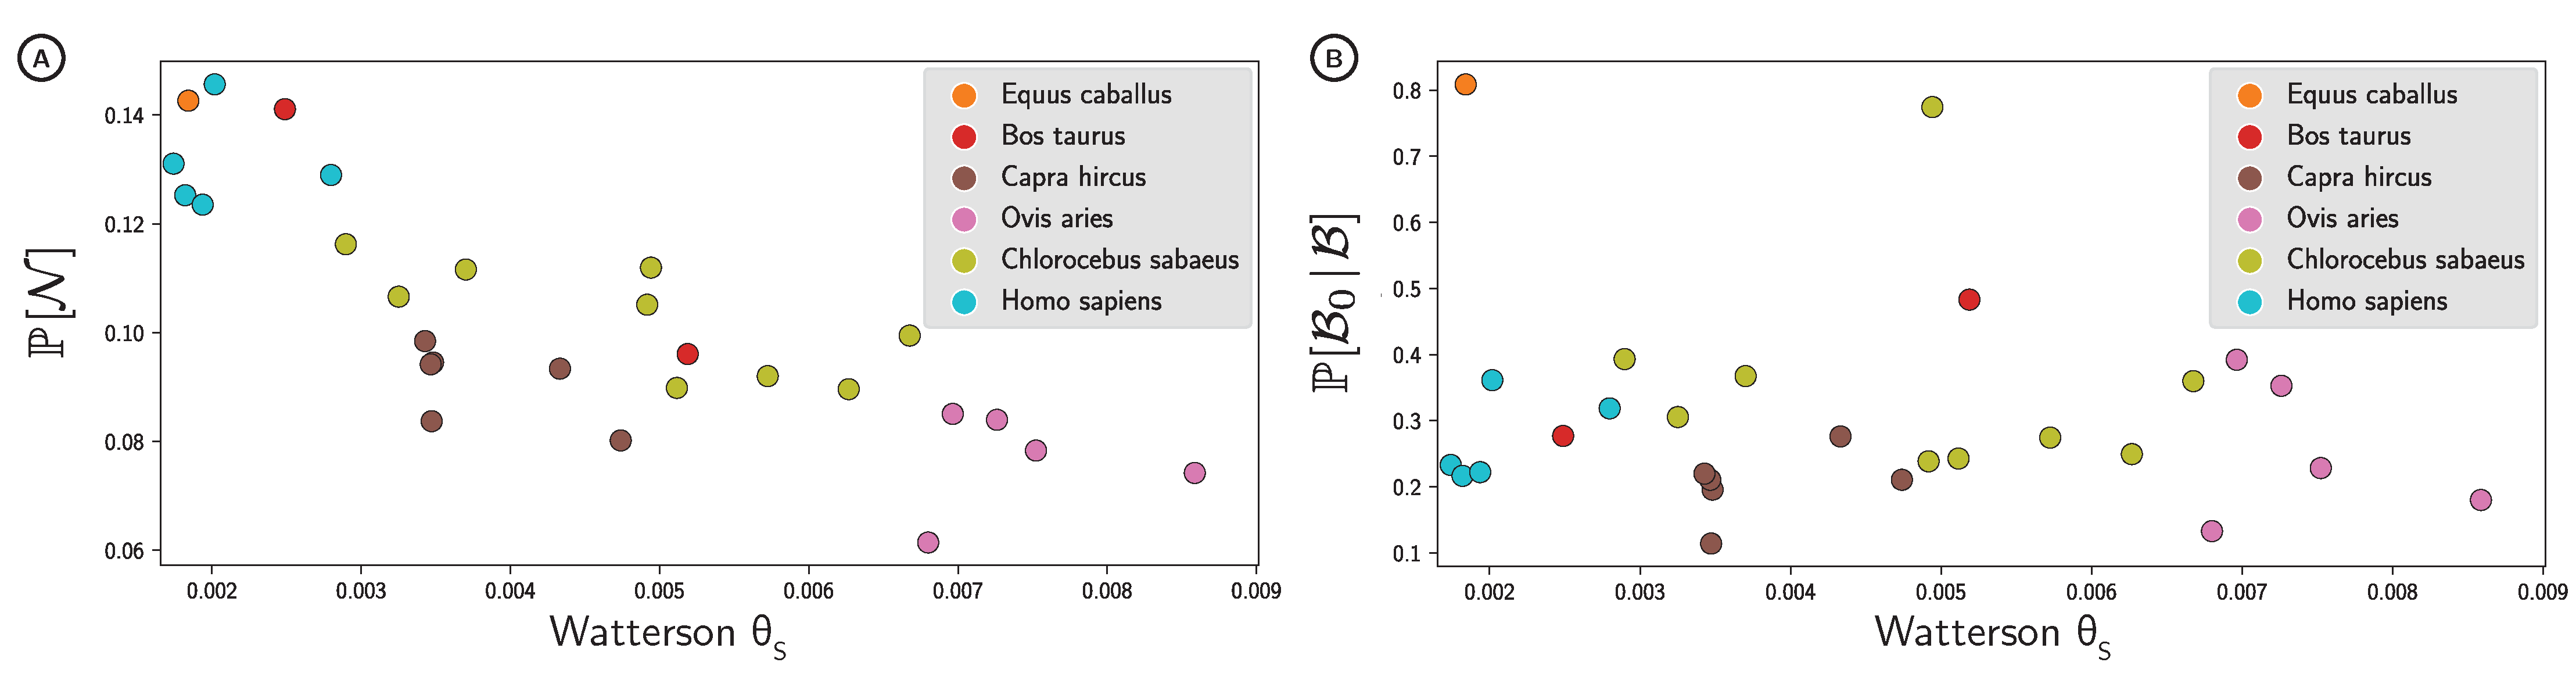
\includegraphics[width=\textwidth, page=1] {artworks/figure.diversity}
        \caption{
            (A) Proportion of nearly-neutral mutations at the population scale ($\proba [ \SpopNeu]$ in the y-axis), shown as a function of the synonymous diversity (Watterson's $\thetaSyn$ in the x-axis).
            (B) Proportion of beneficial back-mutations among all beneficial mutations ($\proba [ \SphyBen  \given  \SpopBen]$ in the y-axis), shown as a function of the synonymous diversity (Watterson's $\thetaSyn$ in the x-axis).
        }
        \label{fig:diversity}
    \end{figure*}

    %\subsection*{The role of epistasis in mammalian protein-coding genes}
    %
    %In our study, we focused on mutations toward a more optimal amino-acid at a given site, assuming that amino-acid fitness landscapes are site-specific and also independent of one another.
    %Contrarily, under epistasis, the fitness effect of a mutation at a particular site depends on the amino-acids present at other sites.
    %Epistasis therefore allows for compensatory mutations, which restore fitness through mutations at loci different from where deleterious mutations take place, and this process also leaves signals interpretable as non-adaptive beneficial mutations~\cite{hartl_compensatory_1996, pollock_strong_2014, starr_epistasis_2016}.
    %Also, epistasis has been shown to play a role in the evolution of protein-coding genes, with amino-acid residues in contact within a protein or between proteins tending to co-evolve~\cite{breen_epistasis_2012, starr_epistasis_2016}.
    %Particularly, the residues in contact co-evolve to become more compatible with each other generating an entrenchment, making empirical evidence for beneficial back-mutations harder to find since restoring mutations becomes less and less likely to occur over time~\cite{goldstein_nonadaptive_2015, goldstein_sequence_2017, park_epistatic_2022}.
    %Nevertheless, the fact that we observe such a high proportion of beneficial back-mutations suggests that the underlying assumptions of our model, namely site-independence, implying no epistasis, and a static fitness landscape, are a reasonable approximation for the underlying fitness landscape of proteins.
    %Our results imply that the fitness effects of new mutations are mostly conserved across mammalian orthologs, in agreement with other studies showing that for conserved orthologs with similar structures and functions, models without epistasis provide a reasonable estimate of fitness effects in protein coding genes~\cite{ashenberg_mutational_2013, youssef_consequences_2020}.

    \subsection*{Detecting adaptation above the nearly-neutral background}

    A long-standing debate in molecular evolution is whether the variations we observe between species in protein-coding genes are primarily due to nearly-neutral mutations reaching fixation by drift or primarily due to adaptation~\cite{kimura_evolutionary_1968,kern_neutral_2018,jensen_importance_2019,gillespie_substitution_1994,Ohta1992}.
    Here we provide evidence that in mammalian orthologs, many substitutions occur through fixation of both deleterious mutations and beneficial back-mutations.
    However, detecting adaptation above this background of nearly-neutral substitutions remains a central question~\cite{kimura_evolutionary_1968,ohta_development_1996}.

    One first strategy is precisely to use a nearly-neutral substitution model as a null model of evolution.
    Under a strictly neutral evolution of protein-coding sequence, we expect the ratio of non-synonymous over synonymous substitutions ($\dnds$) to be equal to one.
    Deviations from this neutral expectation, such as $\dnds > 1$, which can be generated by an excess of non-synonymous substitutions, is generally interpreted as a sign of adaptation.
    However, as shown in this study, a $\dnds > 1$ is not necessarily a signature of adaptation but can be due to beneficial back-mutations.
    So, by relaxing the strict neutrality and assuming a stable fitness landscape instead, one can predict the expected rate of evolution, called $\omega_0$~\cite{spielman_relationship_2015, dosreis_how_2015}.
    Adaptation can thus be considered as evolution under a changing fitness landscape and tested as such by searching for the signature of $\dnds > \omega_0$~\cite{cvijovic_fate_2015, rodrigue_detecting_2017, rodrigue_bayesian_2021}.
    Using a stable fitness landscape as a null model of evolution, thus accounting for selective constraints exerted on the different amino acids, increased the statistical power in testing for adaptation~\cite{latrille_genes_2023}.
    Instead of relying solely on summary statistics (such as $\dnds$ or $\omega_0$), another strategy to detect adaptation is to include changes in the fitness landscapes inherently within the mutation-selection framework~\cite{tamuri_mutationselection_2021}.
    Such mechanistic models could be more general than site-specific fitness landscapes, including epistasis and changing fitness landscapes~\cite{goldstein_sequence_2017, stolyarova_senescence_2020}.

    Here, we have provided empirical evidence that an evolutionary model assuming a stable fitness landscape at the mammalian scale allows us to predict the fitness effects of mutations in extant populations and individuals, acknowledging the balance between deleterious and beneficial back-mutations.
    We argue that such a model represents a null expectation for the evolution of protein-coding genes in the absence of adaptation.
    In that sense, to avoid conflating beneficial mutations with adaptive evolution, the term ``adaptation`` should retain its original meaning associated with a change in the underlying fitness landscape and be modelled as such.

%TC:ignore
    \section*{Acknowledgements}
    \label{sec:acknowledgment}
    We gratefully acknowledge the help of Mélodie Bastian, Nicolas Lartillot, Carina Farah Mugal, Laurent Duret and Nicolas Gambardella for their advice and reviews concerning this manuscript.
    This work was performed using the computing facilities of the CC LBBE/PRABI\@.
    This study makes use of data generated by the NextGen Consortium.
    \textbf{Funding:}
    Université de Lausanne; Agence Nationale de la Recherche, Grant ANR-19-CE12-0019 / HotRec.
    The European Union’s Seventh Framework Programme (FP7/2010-2014) provided funding for the project under grant agreement no 244356 - “NextGen”.
    \textbf{Author contributions:}
    Original idea: T.L.\ and J.J.;
    Model conception: T.L., J.J.\ and N.S.;
    Code: T.L.;
    Data analyses: T.L.\ and J.J.;
    Interpretation: T.L., J.J., D.A.H.\ and N.S.;
    First draft: T.L.\ and J.J.;
    Editing and revisions: T.L., J.J., D.A.H.\ and N.S.
    Project management and funding: N.S\@.
    \textbf{Competing interests:}
    The authors declare no conflicts of interest.
    \textbf{Data and materials availability:}
    The data underlying this article are available at \url{https://doi.org/10.5281/zenodo.7878954}.
    Snakemake pipeline, analysis scripts and documentation are available at \href{https://github.com/ThibaultLatrille/SelCoeff}{github.com/ThibaultLatrille/SelCoeff}.


    \section{Materials \& Methods}
    \label{sec:methods}

    \subsection{Phylogenetic dataset}\label{subsec:phylo-dataset}

    Protein-coding DNA sequence alignments in placental mammals and their corresponding gene trees come from the \href{https://www.orthomam.univ-montp2.fr}{OrthoMaM} database and were processed as in \textcite{latrille_genes_2023}.
    OrthoMaM contains a total of $116$ mammalian reference sequences in v10c~\cite{ranwez_orthomam_2007, douzery_orthomam_2014, scornavacca_orthomam_2019}.
    Genes located on the X and Y chromosomes and on the mitochondrial genome were discarded from the analysis because the level of polymorphism –~which is necessary for population-based analyses~– is expected to be different in these three regions compared to the autosomal genome.
    Sequences of species for which we used population-level polymorphism (see section \ref{subsec:polymorphism-dataset}) and their sister species, were removed from the analysis to ensure independence between the data used in the phylogenetic and population scales.
    Sites in the alignment containing more than 10\% of gaps across the species were discarded.
    Altogether, our genome-wide dataset contains $14,509$ protein-coding DNA sequences in $87$ placental mammals.

    \subsection{Selection coefficient ($\Sphy$) in a phylogeny-based method}
    \label{subsec:s-phylogeny-method}
    We analyzed the phylogenetic-level data using mutation-selection models.
    These models assume the protein-coding sequences are at mutation-selection balance under a fixed fitness landscape characterized by a fitness vector over the $20$ amino acids at each site~\cite{yang_mutationselection_2008, halpern_evolutionary_1998, rodrigue_mechanistic_2010}.
    Mathematically, the rate of non-synonymous substitution from codon $a$ to codon $b$ ($q_{a \mapsto b}^{(i)}$) at site $i$ of the sequence is equal to the rate of mutation of the underlying nucleotide change ($\mu_{a \mapsto b}$) multiplied by the scaled probability of mutation fixation ($\proba_{a \mapsto b}^{(i)}$).
    The probability of fixation depends on the difference between the scaled fitness of the amino acid encoded by the mutated codon ($F_b^{(i)}$) and the amino acid encoded by the original codon ($F_a^{(i)}$) at site $i$~\cite{wright_evolution_1931, fisher_genetical_1930}.
    The rate of substitution from codon $a$ to $b$ at a site $i$ is thus:
    \begin{equation}
        \begin{dcases}
            q_{a \mapsto b}^{(i)} & = 0 \text{ if codons $a$ and $b$ are more than one mutation away,} \\
            q_{a \mapsto b}^{(i)} & = \mu_{a \mapsto b} \text{ if codons $a$ and $b$ are synonymous, and}\\
            q_{a \mapsto b}^{(i)} & = \mu_{a \mapsto b} \dfrac{F_b^{(i)} - F_a^{(i)}}{1 - \e^{F_a^{(i)} - F_b^{(i)}}} \text{ if codons $a$ and $b$ are non-synonymous}.
        \end{dcases}
    \end{equation}
    Fitting the mutation-selection model on a multi-species sequence alignment leads to an estimation of the $4 \times 4$ nucleotide mutation rate matrix ($\UniDimArray{\mu}$) as well as the $20$ amino-acid fitness landscape ($\UniDimArray{F^{(i)}}$) at each site $i$.
    The selection coefficient for a mutation from codon $a$ to codon $b$ at site $i$ is defined as:
    \begin{equation}
        \Sphy^{(i)} (a \mapsto b) = \Delta F^{(i)} = F^{(i)}_{b} - F^{(i)}_{a}.
    \end{equation}
    In our subsequent derivation the source ($a$) and target ($b$) codons as well as the site ($i$) are implicit and thus never explicitly written.
    We used the Bayesian software \textit{BayesCode} (\url{https://github.com/ThibaultLatrille/bayescode}) to estimate the selection coefficients for each protein-coding gene in the mammalian dataset.
    We ran the Markov chain Monte-Carlo (MCMC) algorithm implemented in BayesCode for $2,000$ generations as described in \textcite{latrille_genes_2023}.
    For each gene, after discarding a burn-in period of $1,000$ generations of MCMC, we obtained posterior mean estimates (over the $1,000$ generations left of MCMC) of the mutation rate matrix ($\UniDimArray{\mu}$) as well as the $20$ amino acid fitness landscape ($\UniDimArray{F^{(i)}}$) at each site $i$.

    \subsection{Polymorphism dataset}
    \label{subsec:polymorphism-dataset}

    The genetic variants representing the population level polymorphisms were obtained from the following species and their available datasets: \textit{Equus caballus} (EquCab2 assembly in the EVA study PRJEB9799~\cite{alabri_whole_2020}), \textit{Bos taurus} (UMD3.1 assembly in the NextGen project: \url{https://projects.ensembl.org/nextgen/}), \textit{Ovis aries} (Oar\_v3.1 assembly in the NextGen project), \textit{Capra hircus} (CHIR1 assembly in the NextGen project), converted to ARS1 assembly with dbSNP identifiers~\cite{sherry_dbsnp_2001}), \textit{Chlorocebus sabaeus} (ChlSab1.1 assembly in the EVA project PRJEB22989~\cite{svardal_ancient_2017}), \textit{Homo sapiens} (GRCh38 assembly in the 1000 Genomes Project~\cite{zheng-bradley_alignment_2017}).
    In total, we analyzed 28 populations across the 6 different species with polymorphism data.
    The data was processed as described in \textcite{latrille_genes_2023}.

    Only bi-allelic single nucleotide polymorphisms (SNPs) found within a gene were in our polymorphism dataset, while nonsense variants and indels were discarded.
    To construct the dataset, we first recovered the location of each SNP (represented by its chromosome, position, and strand) in the focal species and matched it to its corresponding position in the coding sequence (CDS) using gene annotation files (GTF format) downloaded from Ensembl (\url{ensembl.org}).
    We then verified that the SNP downloaded from Ensembl matched the reference in the CDS in FASTA format.
    Next, the position in the CDS was converted to the corresponding position in the multi-species sequence alignment (containing gaps) from the OrthoMaM database (see section~\ref{subsec:s-phylogeny-method}) for the corresponding gene by doing a global pairwise alignment (Biopython function pairwise2).
    This conversion from genomic position to alignment position was only possible when the assembly used for SNP-calling was the same as the one used in the OrthoMaM alignment, the GTF annotations, and the FASTA sequences.
    SNPs were polarized using the three closest outgroups found in the OrthoMaM alignment with est-usfs v2.04~\cite{keightley_inferring_2018}, and SNPs with a derived probability lower than 0.99 were discarded (1\% of false positive).

    \subsection{Mutational opportunities}
    \label{subsec:nunber-of-sites}
    The mutational opportunities of any new mutation refer to its likelihood of falling into a specific category (synonymous, deleterious, nearly-neutral, or beneficial).
    Deriving such opportunities is necessary to estimate the strength of selection exerted at the population scale since different categories might have different mutational opportunities, and thus polymorphism and divergence need to be corrected accordingly (see sections~\ref{subsec:substitution-mapping-in-the-terminal-branch},~\ref{subsec:s-polymorphism-method}, and~\ref{subsec:precisison_recall}).
    To calculate mutational opportunities, we reconstructed the ancestral genome of each of the 28 populations, which differs from the corresponding species' reference genome since it accounts for the variability present in the specific population.
    So, for each population, we used the polarized SNPs to reconstruct the ancestral DNA sequence, containing only substitutions and no segregating polymorphisms.
    If an SNP was still segregating in the population, we used its ancestral version.

    From the reconstructed ancestral genome at the base of the population genealogy, all possible mutations were computed, weighted by the instantaneous rate of change between nucleotides obtained from the mutation rate matrix ($\UniDimArray{\mu}$, see section~\ref{subsec:s-phylogeny-method}), summing to $\mu_{\text{tot}}$ across the whole genome, and to $\mu_{\text{syn}}$ when restricted to synonymous mutations.
    Finally, the mutational opportunities for synonymous mutations were computed as the total number of sites across the genome ($L_{\text{tot}}$) weighted by the proportion of synonymous mutations among all possible mutations as:
    \begin{equation}
        L_{\text{syn}} = L_{\text{tot}} \frac{\mu_{\text{syn}}}{\mu_{\text{tot}}}.
    \end{equation}

    Similarly, for non-synonymous mutations, the total mutation rate for each class of selection $\Sphyclass \in \{\SphyDel, \SphyNeu, \SphyBen \}$, called $\mu\left( \Sphyclass \right)$, was estimated as the sum across all non-synonymous mutations if their selection coefficient at the phylogenetic scale is in the class $\Sphy \in \Sphyclass$.
    Accordingly, the mutational opportunities ($L \left( \Sphyclass \right)$) for each class of selection coefficient ($\Sphyclass$) was finally computed as the total number of sites across the genome ($L_{\text{tot}}$) weighted by the ratio of the aggregated mutations rates falling in the class $\mu\left( \Sphyclass \right)$:
    \begin{equation}
        L \left( \Sphyclass \right) = L_{\text{tot}} \frac{\mu\left( \Sphyclass \right)}{\mu_{\text{tot}}}.
    \end{equation}

    Finally, $\proba [ \Sphyclass ]$ is the probability for a non-synonymous mutation to be in the class $\Sphyclass$, thus computed as:
    \begin{equation}
        \proba[\Sphyclass] = \frac{L\left( \Sphyclass \right)}{\sum_{\SphyclassAlt\in \{\SphyDel, \SphyNeu, \SphyBen \} } L\left(\SphyclassAlt \right)}.
        \label{eq:proba-dfe-mutsel}
    \end{equation}

    \subsection{Substitution mapping in the terminal branch}
    \label{subsec:substitution-mapping-in-the-terminal-branch}
    For each gene and each population with polymorphism data available, the genome at the base of the population genealogy was reconstructed (see section~\ref{subsec:nunber-of-sites}).
    We used the ancestral genome reconstructed at the base of the population genealogy and the three closest outgroups found in the OrthoMaM alignment to infer the ancestral protein-coding DNA sequences for each node of the 4-taxa tree by applying the M5 codon model (gamma site rate variation) as implemented in FastML.v3.11~\cite{ashkenazy_fastml_2012}.
    All polarized codon substitutions were then obtained by comparing the ancestral protein-coding DNA sequences before the split from the sister species (closest outgroup) to the genome at the base of the population genealogy.
    We considered \textit{Ceratotherium simum simum} as \textit{Equus caballus'} sister species; \textit{Bison bison bison} as \textit{Bos taurus'} sister species; \textit{Pantholops hodgsonii} as \textit{Ovis aries'} sister species; \textit{Pantholops hodgsonii} as \textit{Capra hircus'} sister species; \textit{Macaca mulatta} as \textit{Chlorocebus sabaeus'} sister species and finally, we considered \textit{Pan troglodytes} as \textit{Homo sapiens'} sister species.
    The selection coefficient ($\Sphy$) of each substitution was then obtained by comparing the difference in amino acid fitnesses for each polarized non-synonymous codon substitution, by referring to the site-specific fitness profile obtained in the phylogeny-based method (see section~\ref{subsec:s-phylogeny-method}).
    Finally, the rate of non-synonymous over synonymous substitutions for a given class of selection coefficient ($\Sphyclass \in \{\SphyDel, \SphyNeu, \SphyBen \}$) was computed as:
    \begin{align}
        \begin{dcases}
            \dn \left( \Sphyclass \right) &= \dfrac{D\left( \Sphyclass \right)}{L \left( \Sphyclass \right)}, \\
            \ds &= \dfrac{D_{\text{syn}}}{L_{\text{syn}}},
        \end{dcases}\label{eq:dnds}
    \end{align}
    where $D \left( \Sphyclass \right) $ was the number of non-synonymous substitutions in class $\Sphyclass$, $D_{\text{syn}}$ was the number of synonymous substitutions across the genome, while $L \left( \Sphyclass \right)$ and $L_{\text{syn}}$ were the numbers of non-synonymous and synonymous mutational opportunities, respectively, as defined in section~\ref{subsec:nunber-of-sites}.
    $\delta(\dnds)$ was computed as the difference between $\dnds$ computed over all substitutions and $\dnds$ when we removed beneficial back-mutations $\dn (\Sphy < 1) / \ds$, normalized by $\dnds$.
    Note that the quantities $\delta(\dnds)$ and $\delta(\dn)$ are equivalent due to the simplification of the factor $\ds$:
    \begin{equation}
        \delta(\dnds) = \dfrac{\dnds - \dn(\Sphy < 1) / \ds}{\dnds} = \dfrac{\dn - \dn(\Sphy < 1)}{\dn} = \delta(\dn).\label{eq:delta-dnds}
    \end{equation}

    \subsection{Scaled selection coefficients ($\Spop$) in a population-based method}
    \label{subsec:s-polymorphism-method}
    To obtain a quantitative estimate of the distribution of selection coefficients for each category of SNPs, we used the polyDFE model~\cite{tataru_inference_2017, tataru_polydfe_2020}.
    This model uses the count of derived alleles to infer the distribution of fitness effects (DFE).
    The probability of sampling an allele at a given frequency (before fixation or extinction) is informative of its scaled selection coefficient at the population scale ($\Spop$).
    Therefore, pooled across many sites, the site-frequency spectrum (SFS) provides information on the underlying $\Spop$ of mutations.
    However, estimating a single $\Spop$ for all sampled mutations is biologically unrealistic, and a DFE of mutations is usually assumed~\cite{eyre-walker_distribution_2006, eyre-walker_estimating_2009}.
    The polyDFE\cite{tataru_inference_2017, tataru_polydfe_2020} software implements a mixture of a $\Gamma$ and exponential distributions to model the DFE of non-synonymous mutations, while synonymous mutations are considered neutral.
    The model estimates the parameters $\DelMean$, $b$, $p_b$ and $\AdvMean$ for non-synonymous mutations as:
    \begin{equation}
        \phi \left( \Spop; \DelMean , b, p_b, \AdvMean \right) =
        \begin{dcases}
            \left( 1 - p_b \right) f_{\Gamma}(-\Spop; -\DelMean, b) & \text{ if $\Spop \leq 0$,} \\
            p_b f_{e}(\Spop; \AdvMean) & \text{ if $\Spop > 0$,} \\
        \end{dcases}
    \end{equation}
    where $\DelMean \leq -1 $ is the estimated mean of the DFE for $\Spop \leq 0$;
    $b \geq 0.2$ is the estimated shape of the $\Gamma$ distribution;
    $0 \leq p_b \leq 1$ is the estimated probability that $\Spop > 0$;
    $\AdvMean \geq 1$ is the estimated mean of the DFE for $\Spop > 0$;
    and $f_{\Gamma}(\Spop; m, b)$ is the density of the $\Gamma$ distribution with mean $m$ and shape $b$, while $f_{e}(\Spop; m)$ is the density of the exponential distribution with mean $m$.

    PolyDFE requires one SFS for non-synonymous mutations and one for synonymous mutations (neutral expectation), as well as the number of sites on which each SFS was sampled.
    For populations containing more than $8$ individuals, the SFS was subsampled down to $16$ chromosomes ($8$ diploid individuals) without replacement (hyper-geometric distribution) to alleviate the effect of different sampling depths in the 28 populations.
    Altogether, for each class of selection ($\Sphyclass \in \{\SphyDel, \SphyNeu, \SphyBen \}$) of non-synonymous SNPs, we aggregated all the SNPs in the selection class $\Sphyclass$ as an SFS.
    The number of sites on which each SFS was sampled is given by $L(\Sphyclass)$ for the non-synonymous SFS and $L_{\text{syn}}$ for the synonymous SFS respectively.
    For each class of selection $\Sphyclass$, once fitted to the data using maximum likelihood with polyDFE, the parameters of the DFE $\left( \DelMean , b, p_b, \AdvMean \right)$ were used to compute $\proba [ \SpopDel \given  \Sphyclass] $, $\proba [ \SpopNeu \given \Sphyclass]$, and $\proba [ \SpopBen \given \Sphyclass]$ as:
    \begin{align}
        \proba [ \SpopDel \given  \Sphyclass] &= \proba [ \Spop < -1 \given \Sphyclass ] = \left( 1 - p_b \right) \int_{1}^{+\infty} f_{\Gamma}(\Spop; -\DelMean, b) \der \Spop, \label{eq:polyProbaDel} \\
        \proba [ \SpopNeu \given \Sphyclass] &= \proba [ -1 < \Spop < 1 \given \Sphyclass ] = p_b \int_{0}^{1} f_{e}(\Spop; \AdvMean) \der \Spop + \left( 1 - p_b \right) \int_{0}^{1} f_{\Gamma}(\Spop; -\DelMean, b) \der \Spop, \\
        \proba [ \SpopBen \given \Sphyclass] &= \proba [ \Spop > 1 \given \Sphyclass] = p_b \int_{1}^{+\infty} f_{e}(\Spop; \AdvMean) \der \Spop. \label{eq:polyProbaAdv}
    \end{align}


    \subsection{\textit{Precision} and \textit{recall}}
    \label{subsec:precisison_recall}
    For readability, we give here \textit{precision} and \textit{recall} for beneficial mutations ($\SphyBen$ and $\SpopBen$), but it can be obtained using the same derivation for the deleterious mutations ($\SphyDel$ and $\SpopDel$) and nearly-neutral mutations ($\SphyNeu$ and $\SpopNeu$).

    \textit{Precision} is the proportion of mutations correctly predicted as beneficial ($\proba [ \SpopBen \cap  \SphyBen]$) out of all predicted as beneficial back-mutations ($\proba [ \SphyBen]$), which can be written as a conditional probability:
    \begin{equation}
        \frac{\proba [ \SpopBen  \cap  \SphyBen]}{\proba [ \SphyBen]} = \proba [ \SpopBen  \given  \SphyBen].
        \label{eq:precision}
    \end{equation}
    Namely, \textit{precision} corresponds to the probability for a back-mutation ($\SphyBen$) to be effectively beneficial at the population level ($\SpopBen$).
    This probability, computed from eq.~\ref{eq:polyProbaAdv}, is obtained by restricting our analysis to SNPs that are predicted to be beneficial back-mutations (yellow fill for the category $\SphyBen$ in fig.~\ref{fig:homo-afr-results}D).

    \textit{Recall} is the proportion of mutations correctly predicted as beneficial ($\proba [ \SpopBen \cap  \SphyBen]$) out of all beneficial mutations ($\proba [ \SpopBen]$), which can be written as a conditional probability:
    \begin{equation}
        \frac{\proba [ \SpopBen \cap  \SphyBen]}{\proba [ \SpopBen]} = \proba [ \SphyBen  \given \SpopBen ].
    \end{equation}
    Namely, \textit{recall} corresponds to the probability for a beneficial mutation at the population level ($\SpopBen$) to be a beneficial back-mutation ($\SphyBen$).
    Using Bayes theorem, \textit{recall} can be re-written as:
    \begin{equation}
        \proba [\SphyBen \given \SpopBen] = \frac{\proba [\SpopBen \given \SphyBen] \times \proba[\SphyBen]}{\ProbaPopBen},
        \label{eq:bayes}
    \end{equation}
    where $\proba [\SpopBen \given \SphyBen]$ and $\proba [ \SphyBen ]$ can be calculated using equations~\ref{eq:precision} and~\ref{eq:proba-dfe-mutsel}, respectively, and $\proba [ \SpopBen ]$ is the probability of a mutation to be beneficial at the level of the population, which can be computed from the law of total probabilities as:
    \begin{equation}
        \proba [ \SpopBen ] = \sum_{\Sphyclass \in \{\SphyDel, \SphyNeu, \SphyBen \} }\proba [\SpopBen \given \Sphyclass ] \times \proba [\Sphyclass ].
        \label{eq:total_proba}
    \end{equation}
    \printbibliography
\end{document}
%TC:endignore